\documentclass{sig-alt-release2}
\usepackage{url}
\usepackage{hyperref}
\usepackage{color}
\usepackage{graphics,graphicx}

\usepackage{epsfig}
\usepackage{epstopdf}

\usepackage{colortbl}
\usepackage{multirow}
\usepackage{booktabs}
\usepackage{ifthen}  

\graphicspath{ {./img/} }

\begin{document}
\newcommand{\todo}[1]{\textcolor{red}{#1}}
\def\newblock{\hskip .11em plus .33em minus .07em}

\conferenceinfo{DIM3} {2010, Glasgow, UK} 
\CopyrightYear{2010}
\clubpenalty=10000
\widowpenalty = 10000

\title{DIM3 Web Application Report}

\numberofauthors{3}
\author{
\alignauthor
Ross Eric Barnie, \\
Craig Cuthbertson, \\
Ross Taylor \\
\affaddr{Just. No.}\\
\affaddr{{DIM3}}\\
\affaddr{0901758, 1002386, 1002858}\\
\email{
  0901758b@student.gla.ac.uk\\
  1002386c@student.gla.ac.uk\\
  1002858t@student.gla.ac.uk\\
}
}
\maketitle

\begin{abstract}
Provide a concise summary of the design of the application

\end{abstract}

\section{Aim of Application}
\begin{itemize}
\item	What is the purpose of the application?
%\item	Eg. The application is an academic search engine called AcaSe and is it is based upon the PuppyIR Framework\cite{glassey2011framework}, which has been used to construct other such services\cite{glassey2010fifi,elliot2010fifi}. The main purpose of this web application is to provide a customized interface to services such as Google Scholar and MS Academic Search. 
\item	What are the assumptions about the aims and objectives?
\item	Describe the design goals and objectives of the application.
\item	What are the constraints of the project?
\item	Functionality List: i.e. what is the required and desired functionality?
\item	Reflective Questions: 
\item	Is the scope of the application appropriate? 
\item	Are the design goals realistic/achievable? 
\item	How complex is the application? 
\item	Is distribution across the web appropriate? 
\end{itemize}

\section{Client Interface}
\subsection{Wireframe Designs}
\subsubsection{Login/Main Page}
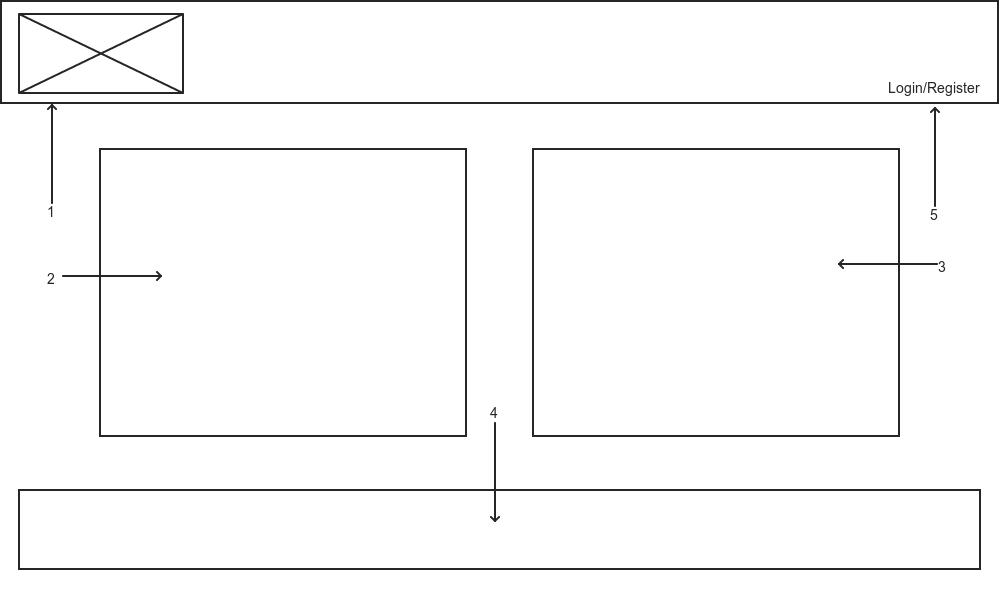
\includegraphics[scale=0.3]{img/login}
\begin{enumerate}
\item \textbf{Logo Header} - A constant feature running throughout all areas of the system. This is clickable and will return the user to the homepage from any page in the website.
\item \textbf{Login Window} - A form to provide users with login functionality will be included here.
\item \textbf{Register Window} - A form to allow users to register will be included here.
\item \textbf{Popular Playlists} - This section will include popular playlists. Playlists popularity will be assessed by click count over the time period of one week.
\item \textbf{User Controls} - This section will include controls relevant to the user. In the case of a user that has not yet logged in, this will display Login/Register with links to each.
\end{enumerate}

\subsubsection{Logged In/Main Page}
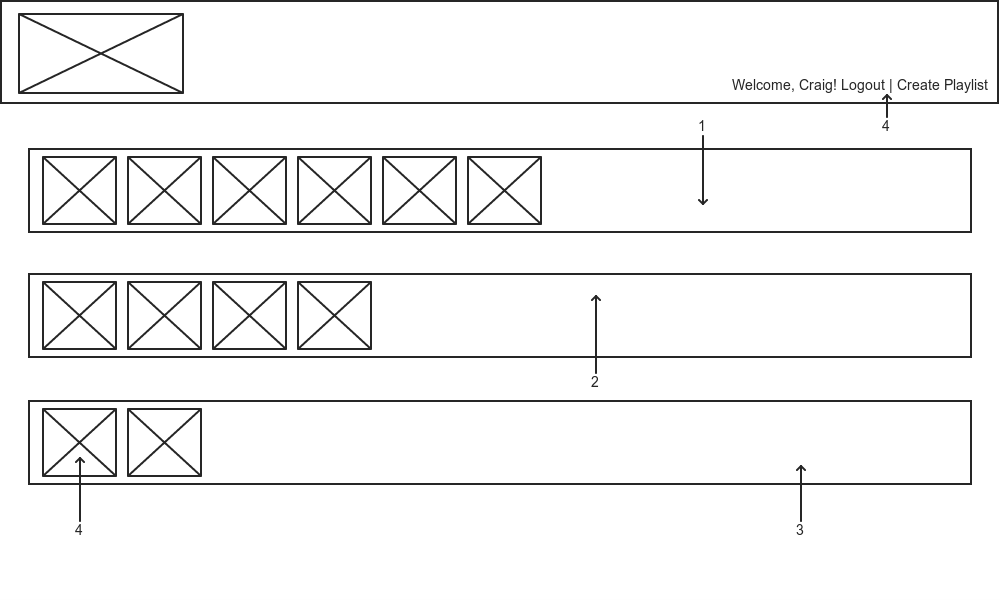
\includegraphics[scale=0.3]{img/loggedin}
\begin{enumerate}
\item \textbf{My Playlists} - User created playlists will be displayed here.
\item \textbf{Collaborated Playlists} - Playlists the user has collaborated on will be displayed here.
\item \textbf{Popular Playlists} - Popular playlists will be displayed here.
\item \textbf{Playlist Thumbnail} - A thumbnail will be generated from a selection of thumbnails of media included in the playlist.
\item \textbf{User Controls} - This section includes controls relevant to the user. In the case of a user that has logged in, this will display a link to the users profile, Logout and Create Playlist.
\end{enumerate}

\subsubsection{Create New Playlist}
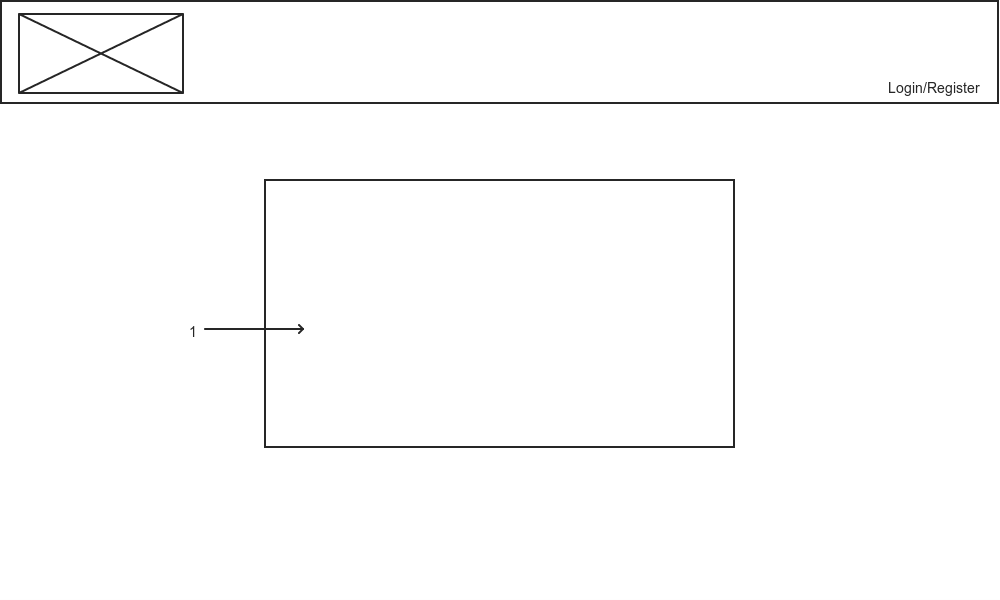
\includegraphics[scale=0.3]{img/new_pl}
\begin{enumerate}
\item \textbf{Create new playlist form} - This section will include a form to create a new blank playlist.
\end{enumerate}

\subsubsection{View Playlist}
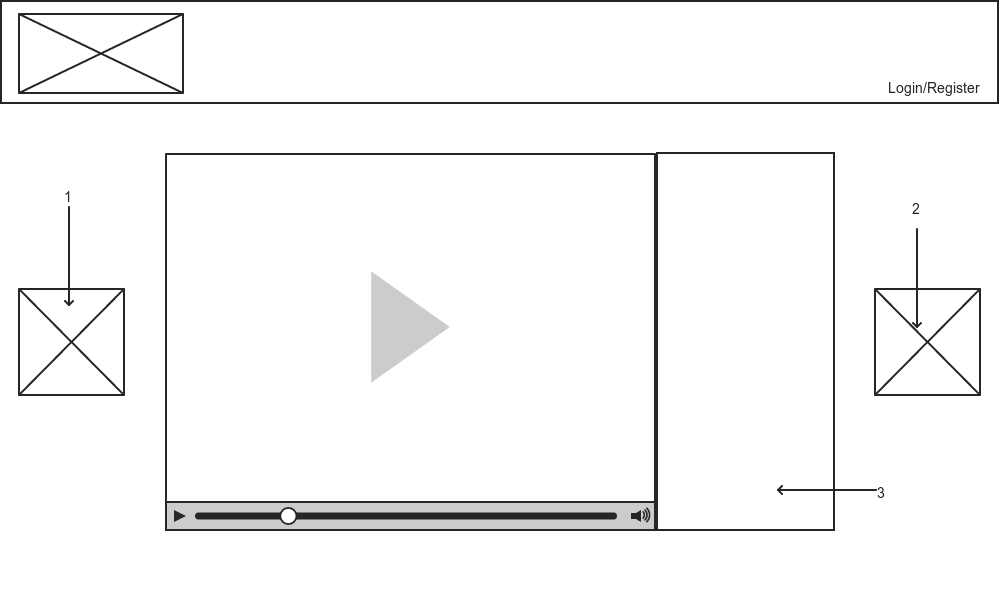
\includegraphics[scale=0.3]{img/playlist}
\begin{enumerate}
\item \textbf{Previous} - Will display a thumbnail of the previous media item in the playlist. Clicking this will play the previous item in the playlist.
\item \textbf{Next} - Will display a thumbnail of the next media item in the playlist. Clicking this will play the next item in the playlist.
\item \textbf{Media Player} - This section will contain the media applet that will play the media. 
\item \textbf{Playlist Details} - This section will contain details retaining to the playlist, including the playlist title, author, and a form to add a new media item to the playlist (if playlist is the users' own/public).
\end{enumerate}

\subsubsection{User Profile}
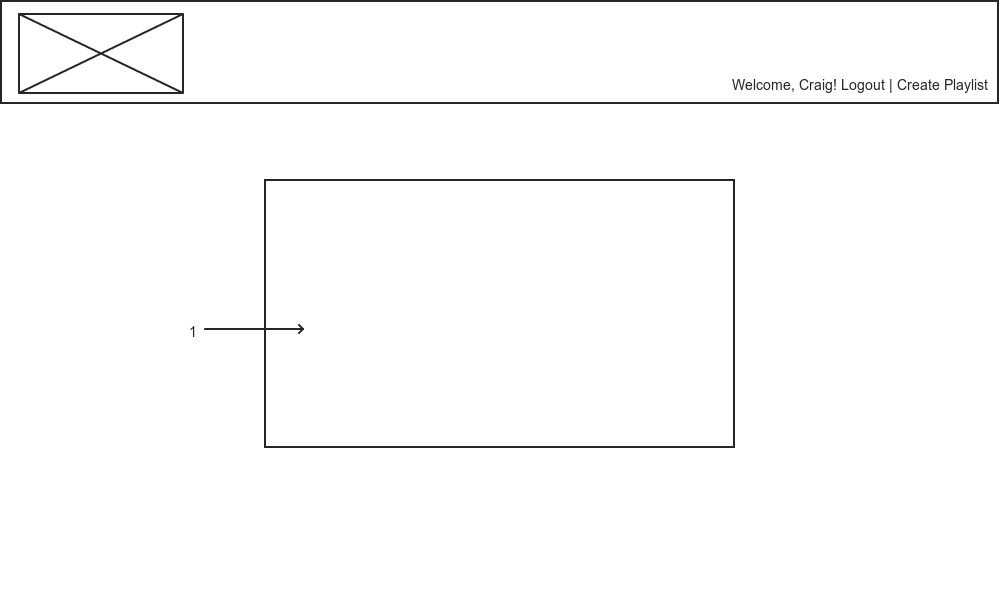
\includegraphics[scale=0.3]{img/userprof}
\begin{enumerate}
\item \textbf{Profile View} - This section will contain details retaining to a users' profile, such as any playlists the user is assosciated with (own/collaborated).
\end{enumerate}

\subsection{Use Cases}
\subsubsection{Individual User}
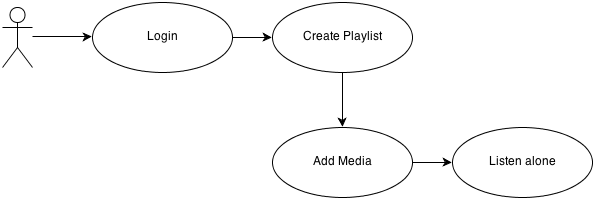
\includegraphics[scale=0.3]{img/uc_listenalone}
\subsubsection{Collaborative Playlist}
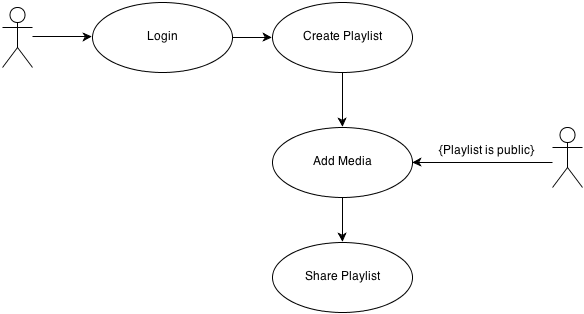
\includegraphics[scale=0.3]{img/uc_share}

\subsection{Dynamic Interface Components}
Due to the nature of the system, it requires many dynamic interface components. 

\subsubsection{Playlist Viewer}
The most prominent of which appear on the playlist page. The playlist page must be able to dyanmically update the content of the media container based on a number of conditions.
\begin{itemize}
\item Media ends
\item Media is skipped forward
\item Media is skipped backward
\end{itemize}

In all three of the above cases, code must execute to update the display elements to show relevant data.
\begin{itemize}
\item Playing media must be replaced with new media
\item Forward and back thumbnails must be replaced with new forward/back thumbnails
\end{itemize}

A dynamic interface is also required in this instance to prevent unauthorised users from adding media to playlists.

\subsubsection{Index Page}
The index page must be updated according to whether a user is currently logged in. This will prevent users who are already logged in from seeing unneccesary controls; and allow the system to display data tailored to the currently logged in user - such as playlists a user has contributed to. 

\subsection{Dynamic Update Calls}
All calls to dynamically update content were written in JavaScript.

The calls implemented are as follows.

\begin{itemize}
\item \textbf{onPlayerReady(event)} - Initialises player
\item \textbf{stopVideo()} - Stops the video playing (youtube API)
\item \textbf{onPlayerStateChange(event)} - Calls when the video stops playing. Calls nextVid()
\item \textbf{nextVid()} - Loads next video
\item \textbf{nextImg()} - Loads thumbnail images for previous and next media
\end{itemize}

\subsection{How the Interface helps}
The user interface has been designed so as to guide the user through each stage required to create and view a playlist. Once the user completes one action, the interface will redirect the user to the next screen they will be likely to use. By doing this, users will waste minimal time trying to navigate menus. 

The user interface is clear as to what data is required of the user at all times. This will help the user to instantly know what information they must locate and include. 

The user interface is kept consistent, and each page follows a general layout structure. This makes the system more intuitive as the user is able to guess where controls will be if a screen looks similar to one they have seen before.

\subsection{Appeal of User Interface}
The user interface has been designed to be as appealing as possible. At its current state, some tidying up of the CSS is still required, however, pages have been designed to minimize cluttering and graphics have been used to add to the appeal.
The media player itself has been to take up as much of the page as possible. This is to draw focus to it, as the current playing media is the main aspect of the website. 
The website is also kept consistent throughout the pages, with a similar look and feel. This makes the website intuitive to the user, as users are likely to be able to guess the location of functions before they have loaded.

\subsection{Client Technologies Used}
The only prerequisite of a client wishing to use the system is to have a 'modern' web browser. The application uses CSS, JavaScript, Flash (for some media applets) and HTML - all of which are available through most browsers. 

These technologies were chosen as we wanted to make the system as accessible to as many users as possible. We invisaged this application going mainstream and therefor wanted minimal fuss. These technologies were examined to assess their suitability to implement the system to a high standard, and were deemed acceptable.

Another solution that could of been implemented was to write the entire program in Flash/C/Java. Although suitable, these would require the user to install extra software which we felt would not be suitable.
\section{Application Architecture}
\begin{itemize}
\item	N-Teir Architecture Diagram
\item	i.e. data flow diagram between the interface/client, middle ware, and backend services/data repos
\item	Describe the data model i.e. what data needs to be stored or persisted by the application?
\item	What are the relationships within the data model.
\item	i.e. use ER diagram and explain.
\item	Describe the backend services used (if any).
\item	Reflective Questions: 
\item	How have you ensured that there is a separation of concerns? 
\item	What other technology could have been used instead of django? 
\item	What are the advantages of using a Web Application Framework over other technology? 
\item	And, what are the disadvantages?
\end{itemize}

\begin{figure}[h]
  \begin{center}
    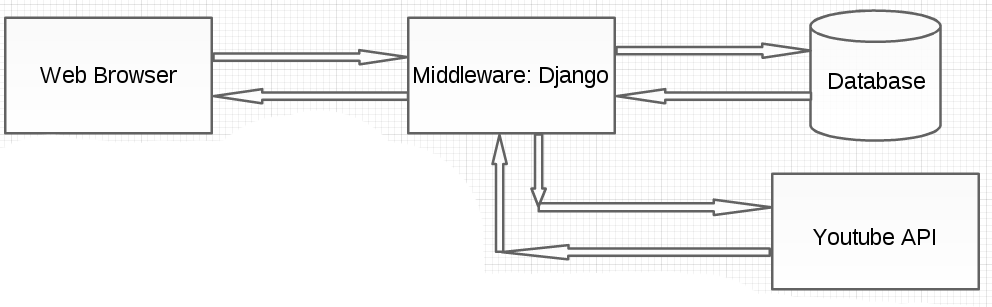
\includegraphics[width=0.45\textwidth]{ntier}
    \caption{N-Tier Diagram} \label{fig:n-tier}
  \end{center}
\end{figure}

\begin{figure}[h]
  \begin{center}
    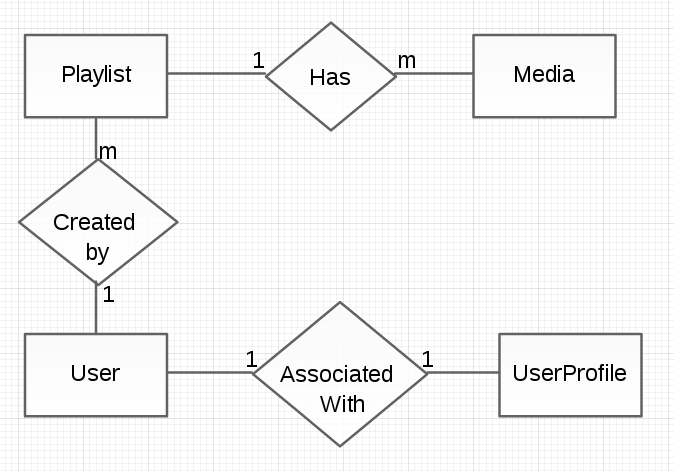
\includegraphics[width=0.45\textwidth]{ER}
    \caption{Entity-Relationship Diagram} \label{fig:ER}
  \end{center}
\end{figure}




\section{Message Parsing}
\begin{itemize}

\item	On the architecture diagram, Identify and label the main messages that will be parsed through the application.
\item	or alternatively (and preferably) include sequence diagrams to denote the sequence of communications parse between clients and servers.
\item	Describe the messages that are parsed back and forth through the application.
\item	For the main transactions - describe the payload of the messages 
\item	i.e. What are the contents of the messages? i.e. include sample XML, XHTML, JSON, etc of one or two messages.
\item	What is the format of the messages? 
\item	Why this format? 
\item	What other formats could be used, what are the advantages and disadvantages of these other formats?
\end{itemize}

%%%%%%%%%%%%%%%%%%%%%%%%%%%%%%%%%%%%%%%%%%%%%%%%%%%%%%%%%%%%%%%%%%%%%%%%

\section{Implementation Notes}

\subsection{Views}
%\item Views - What are the main views that you have implemented and what do they do?

The main views we created for the project were as follows:

\begin{itemize}
\item Index - This view loads the index.html template and populates it with data for the current user. It gets a list of all of the playlists and then gets a seperate list of playlists which created by the current user. This view also deals with registering users and logging users in by saving the data entered into the relevant form on the index page.
\item Playlist - The playlist view deals with the add\verb=_=media function by verifying the form passed to the function is valid, extracting the data from the form and then performing the appropriate function calls to add the media to the database. This view also populates the context dictionary with the correct media when the playlist page is opened.
\end{itemize}

\subsection{URL Mapping Schema}
%\item URL Mapping Schema - what is your URL mapping and schema?

The URL mapping schema we decided to use was designed to be fairly easy to read and aquire information from. Every URL begins with the IP then `/allthemedia/'. The next section contains information about the type of page the user is accessing, for example `/login/', `/register/', `/about/', `/user/' etc. If this section contains `/user/' then the user is accessing a page with information relating to a specific user. This is followed by `/user/[username]/' to view the user profile of a particular user. This can be followed by a playlist title to view a playlist created by the specified user i.e. `/allthemedia/user/joe/coolsongs/' would display the playlist called `coolsongs' which was created by the user called `joe'. Anything beyond this stage specifies actions to be performed on a particular playlist, such as add\verb=_=media.

\subsection{External Services}
%\item External Services  - what external services does your application include and what handlers did you include?

The main external service used by our application is YouTube. This is used extensively by our 'Playlist' page, the main feature of which is a large YouTube player which plays the playlist media. This is created using the YouTube API which then displays the media from the current playlist.

\subsection{Functionality}
%\item	Functionality Checklist (which functionality is completed)

The folowing functionality is completed:

\begin{itemize}
\item Login/Logout/Register
\item Create playlists
\item View playlists
\item Adding media to a playlist from the 'add\verb=_=media' page
\item Auto-playing videos in a playlist
\item Skipping forwards and backwards through a playlist
\end{itemize}

%\item	Known Issues (what kind of works, what kind of errors to do you get)

The following functionality is unfinished, buggy or unimplemented:

\begin{itemize}
\item Adding to a playlist from the form on the playlist page - currently re-loads the playlist page with no playlist loaded and without adding the new media.
\item CSS missing from add\verb=_=media page - we had intended to add media from the playlist page and the add\verb=_=media was supposed to be a temporary page. However, because this feature remains unfinished, the add\verb=_=media page is the only way to add media to a playlist.
\item After adding media to a playlist the re-direct goes to an empty playlist page with an incorrect URL.
\item Adding media from sites other than YouTube is not currently supported.
\item Collaborative playlist editing and Popular Playlists - unimplemented due to time constraints.
\end{itemize}

\subsection{Technologies Used}
%\item What technologies have been used and are required for the application. Include a list or table of all the technologies, standards, and protocols that will be required.

For the implementation of this application we used the following technologies:

\begin{itemize}
\item Django - Django is the web application framework we used. This deals with a lot of the passing of data between pages and between the client and the server.
\item Python - We used Python to write the files used by Django which define components such as the views, the models and the URL schema. 
\item HTML - Used to write the page templates.
\item JavaScript - A number of scripts are used in the page templates, for example: the generation of the YouTube player on the playlist page is done within a script.
\item CSS - The appearance and layout of the pages is handled using CSS.
\item YouTube API - The YouTube API is accessed by the playlist page to allow our application to view YouTube videos and also to tell when the videos are finished to autoplay the next video.
%\item Amazon Servers - *************************************************
\end{itemize}

%%%%%%%%%%%%%%%%%%%%%%%%%%%%%%%%%%%%%%%%%%%%%%%%%%%%%%%%%%%%%%%%%%%%%%%%

\section{Reflective Summary}
Personally, I feel as though I have learnt quite a lot during the course of the project. Although I used to be extensively involved in web development, having never used a framework before, it was a new and interesting experience having to edit several different - seemingly unrelated - files to create the desired look and feel of the application. The concept of having forms show up in a standard layout was also an interesting one, and I learned a lot about the flow of data through a django website, and where different aspects of it came from.

Due to personal previous experience, the application framework was quite a hinderance to the progress of the project as I constantly found myself wanting to edit the top level code rather than the code that would generate a certain form/object. This, I assume, is all down to habit though - and I can definitely see the benefit in forcing a standardisation of objects such as forms. 
The administration interface was quite useful to development meaning it was not necessary to delve deep into the raw database. Though, again, I found myself wanting complete control.

All major problems encountered were due to the limiting nature (or my inexperience) of django. Countless days were spent trying to get a model to pass a form through it whilst also accepting another form's input. In the end, some modules were left without this complete integration which I am extremely disappointed about. 

In the end, I would say the major achievements in the project were the things we worked hardest for - such as solving our earlier problems with forcing models to accept more than one input. The system was also completed (almost error-free) in an extremely limited timespan, something which I am incredibly proud of. The stylesheet was written from scratch, meaning our system will be different to every other system out there and I believe we have made our initial idea all those weeks ago a reality. 

%%%%%%%%%%%%%%%%%%%%%%%%%%%%%%%%%%%%%%%%%%%%%%%%%%%%%%%%%%%%%%%%%%%%%%%%

\section{Summary and Future Work}

\subsection{Summary}
%\item	Summary of application and its current state.
%\item	Include a list or table of all the technologies, standards, and protocols that will be required.
%\item	What are the limitations?

To summarise, our application currently functions as a video playlist system for Youtube videos. Users can register and log in which allows playlists to be saved and linked to a particular user. The user who created the playlist can also add more videos to the playlist. When a playlist is being viewed the videos will auto-play in order when each video ends. Users can also skip forwards and backwards through the playlist. The videos in the playlist will loop forever, provided the playlist which has been chosen contains videos.

Currently, adding to playlists can only be done through the add\verb=_=media page and not from the playlist page as had been planned. Another limitation of the application in its current state is that only the creator of a playlist can add to it as opposed to our original idea which was to have multiple users able to collaborate on one playlist. We would also ideally have allowed users to remove media from playlists but this feature in unimplemented. The main limitation is that only media from YouTube is currently supported. We had initially intended for users to be able to add media from multiple sources but this wasn't implemented as it took us longer than we had originally expected to integrate the YouTube API.

\subsection{Future Work}
%\item Plans for future development
Given the limitations noted previously, there is plenty of scope for improvement and expansion of this application. One key feature we would have liked to integrate is support for media from multiple sources, not only YouTube. We had originally looked at sites such as GrooveShark and Soundcloud, however, streaming using the GrooveShark API requires you to pay so we decided this was not feasible. We would still like to include support for Soundcloud and similar services and may do so in the future.

Another feature we would like to implement in the feature would be the collaborative playlist editing as this was one of the features we liked the most when we first had the idea for the project. If this was implemented we would also need to add the ability for creators to remove videos from their playlists to prevent other users ruining their playlists.

\section{Acknowledgements}
Our thanks to the lecturers and demonstrators for their comments and
suggestions.
We would also like to thank the industry panel members for their
comments and for taking the time to witness our demonstration.

\bibliographystyle{abbrv}
\bibliography{bibliography}

\end{document}
